% section 4
% Kota Miura (miura@embl.de)

\section{Segmentation}
\label{sec:segmentation}

Segmentation refers to the process in which an image is subdivided into
constituent regions or objects. These objects can be further
processed or analyzed for the extraction of quantitative information.
Biological image data is usually messy and noisy, and as a result
difficult to be segmented properly. Multiple image pre-processing steps are
often required to allow a good segmentation. We often combine segmentation
with various morphological processing and filtering techniques (such as the ones described in the previous section) to achieve an accurate and robust
segmentation.
Image segmentation algorithms are generally based on one of the two basic
properties of intensity values: discontinuity and similarity. In the
first category, the approach is to partition an image based on abrupt
changes in intensity, edge-detection algorithms falls in this category. In the second approach, an image is partitioned into
regions that are similar according to set of predefined criteria.
Thresholding and watershed segmentation fall in this category.

\subsection{Thresholding}
\label{sec:Thresholding}
Many biological images comprise of light objects over a constant dark
background (especially those obtained using fluorescence microscopy),
in such a way that object and background pixels have gray levels
grouped into two dominant modes. One obvious way to extract the objects
from its background is to select a threshold T that separates these
modes:

\begin{equation}
g(x,y)= 
\begin{cases}
1 & \text{if $f(x, y) > T$}\\
0 & \text{otherwise}
\end{cases}
\end{equation}

Where $g(x,y)$ is the thresholded image of
$f(x,y)$.

In a sense, thresholding is an extreme case of contrast enhancement we
studied already (\ref{subsec:enhancecontrast}). By setting a threshold value $T$ and
converting the image, pixels with values above $T$ becomes white and
otherwise black (color could be in inverse). 

Image thresholding operation turns the image into a black and white image
which is called \textit{binary image}\footnote{Some of \ijmenu{[Process{\ldots}]}operations work only with binary images, so thresholding is a prerequisite for those filters}.

\begin{indentexercise}{1}
Although there is a function specialized for
the thresholding, we first try thresholding images using
\ijmenu{brightness / contrast} function
we used in the previous section. Open the image \textbf{2D\_Gel.jpg}.
Then \ijmenu{[Image > Adjust > Brightness/Contrast]}. 
In "B\&C" contrast control window, set the "minimum" and "maximum" to a same value. You then should
see that the LUT curve is vertical, like shown in Fig.~\ref{fig:img106} below. Then
change the brightness: this will change the x-position of the vertical
LUT, and at the same time, you will see the ratio of black and white
area changes. This corresponds to the changing of thresholding value.


%figure
\begin{figure}[htbp]
\begin{center}
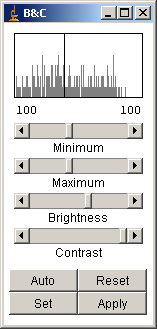
\includegraphics[width=4cm]{fig/CMCIBasicCourse201102-img106.png}
\caption{ Thresholding by using Brightness/Contrast Control Dialog.}
\label{fig:img106}
\end{center}
\end{figure}
\end{indentexercise}
 
Thresholding could be also done by setting two threshold values, lower
limit and upper limit: which means that pixels with a certain range of
values could be selected. This operation is sometimes called
"density slice". We then have a new rule as follows, with lower threshold value $T_1$ and upper threshold value $T_2$.

\begin{equation}
g(x,y)= 
\begin{cases}
1 & \text{if $T_2 > f(x, y) > T_1$}\\
0 & \text{otherwise}
\end{cases}
\end{equation}

\begin{indentexercise}{2}
Open the image \textbf{2D\_Gel.jpg} (or
revert the image to the original by \ijmenu{[File > Revert]} if you still have the image used in the precious exercise).
Then do \ijmenu{[Image > Adjust > Threshold\ldots]}. 
You will see that the Gel image is automatically
thresholded. The area highlighted in red is where pixels with value
lower larger than 0 and lower than 149. In the
"Threshold" window, the range of values that is highlighted is shown by red rectangular frame over the
histogram. Try changing the upper and lower threshold value using the
sliding bar below and study the effects on highlighted area in image. 

%figure
\begin{figure}[htbp]
\begin{center}
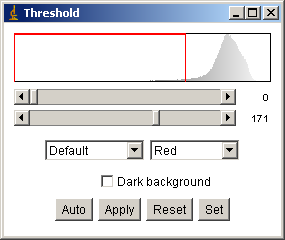
\includegraphics[width=7cm]{fig/CMCIBasicCourse201102-img107.png}
\caption{ Thresholding Dialog.}
\label{fig:img107}
\end{center}
\end{figure}

\ijmenu{Set} button in the threshold
window enables to you input the lower and upper threshold numerically.
The original image file is not altered until you click the button
\ijmenu{Apply} at the bottom of the
threshold window. Click \ijmenu{Apply}, and
check the result of conversion by saving it as a text file, or simply
by checking the pixel values using the value indicator in the status
bar. 
\end{indentexercise}

Instead of manually setting the threshold level, many algorithms for
automatically setting the threshold level exist.
\ijmenu{Auto} button in the threshold
window is one of these automatic thresholding algorithms. Various
algorithms for automatic determination of threshold value are available
(such as Otsu, Maximum Entropy and so on) and you could choose one of
them by the drop-down menu on the left side. Following is a list of
available Algorithms:


\begin{itemize}
\item IsoData
\item Maximum Entropy
\item Otsu
\item Mixture Modeling
\item Huang
\item Intermodes
\item Li
\item Mean
\item MinError
\item Minimum
\item Moments
\item Percentile
\item RenyiEntropy
\item Shanbhag
\item Triangle
\item Yen
\end{itemize}

For choosing an algorithm, a proper way might be to look for original papers
describing the algorithm and think which one would work best for your
purpose (!), but in practice, you could try one by one and just choose one
that fits your demand. Instead of manually trying out all available algorithms, you could test them in one action by \ijmenu{[Image > Adjust > Auto Threshold]} and then choose ``Try All'' in the dialog window (fig. \ref{fig:thresholdTryAll})


\begin{figure}
\begin{center}
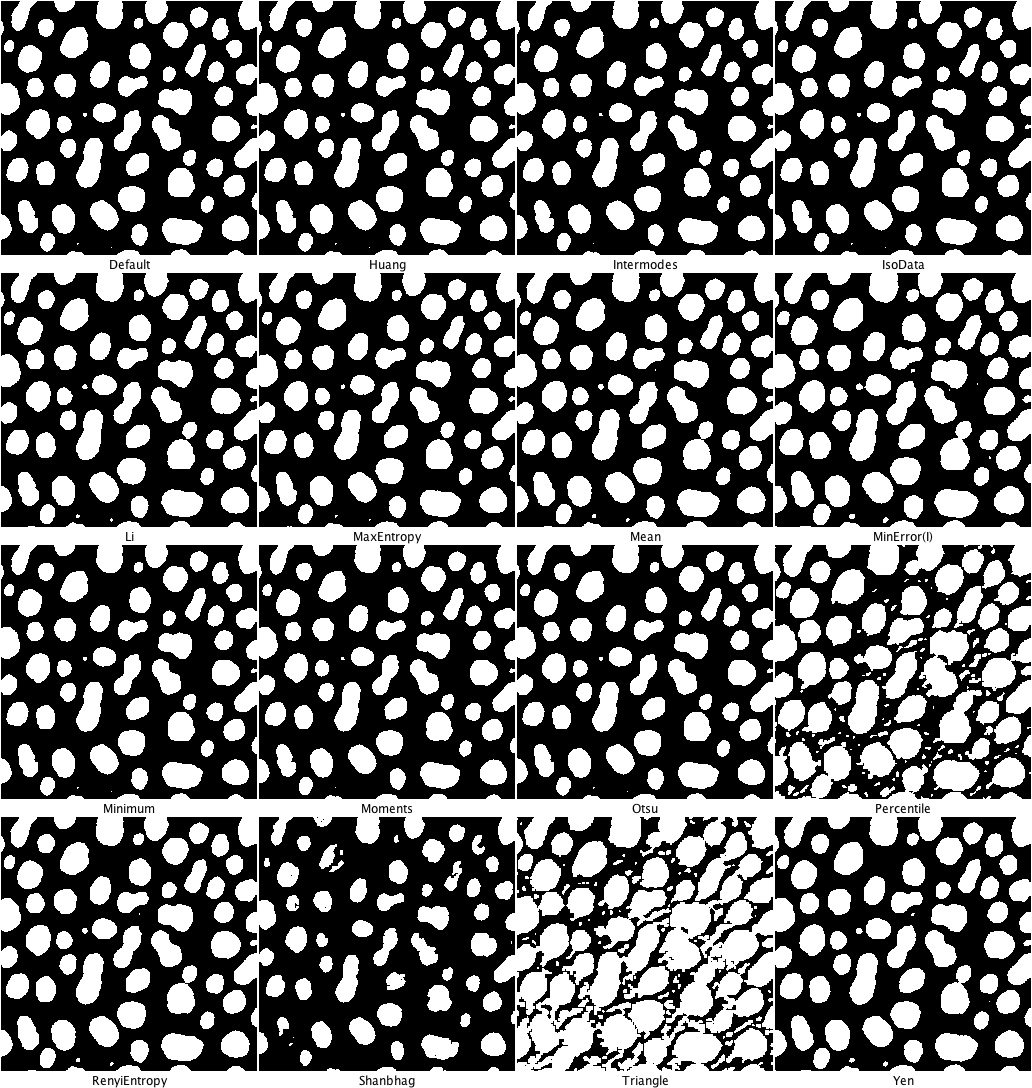
\includegraphics[width=0.9\textwidth]{fig/ThresholdTryAll.png}
\caption{For testing all algorithms, ``try all'' choice in AutoThreshold dialog is convenient. The image above is an output of doing this with the image blob.tif. Algorithm names are printed in small fonts below each image.} 
\label{fig:thresholdTryAll}
\end{center}
\end{figure}

In batch processing, command for automatic threshold would be like this:

\ilcom{setAutoThreshold("Huang dark");}

The first argument is the name of the algorithm and could be any of the
ones listed above.
 
\subsection{Feature Extraction - Edge Detection}

Patterns within an image have features such as lines and corners. To detect them we employ a procedure called ``Feature Extraction''. In the general sense, this means to extract certain objects that you are focusing on. In a strict definition in image processing, this means to do some defined calculations with neighboring pixels to get a feature image. This output then can be used simply for segmentation, but also for machine learning based automatic classificaiton (we will try this technique in a later section). 

The edge detection was already mentioned in the find edge kernel section (\ref{subsub:findedgekernel}). Edge detection is one of those feature extractors and is useful for segmenting object edges. 
In the ImageJ menu we could use commands 
\begin{itemize}
\item \ijmenu{[Process > Find Edges]} (uses Sobel kernel) or 
\item \ijmenu{[Plugins > Feature Extraction > FeatureJ > FeatureJ Edge] (uses gradient filter)} 
\end{itemize}
that do the job but here we try to do it step by step, starting from manually preparing Sobel kernels. We process an image of microtubule filament. 

\begin{indentexercise}{1}
Open image microtubule.tif. We expect that the values will exceed 255 (8-bit) so convert the image to
32-bit by \ijmenu{[Image > Type > 32-bit]}. To apply Sobel kernel in x and y direction, duplicate the image by \ijmenu{[Image Duplicate\ldots]}. 
To the original image apply convolution in x-axis. 
Do \ijmenu{[Process > Filter > Convolve]} and input the following kernel:

%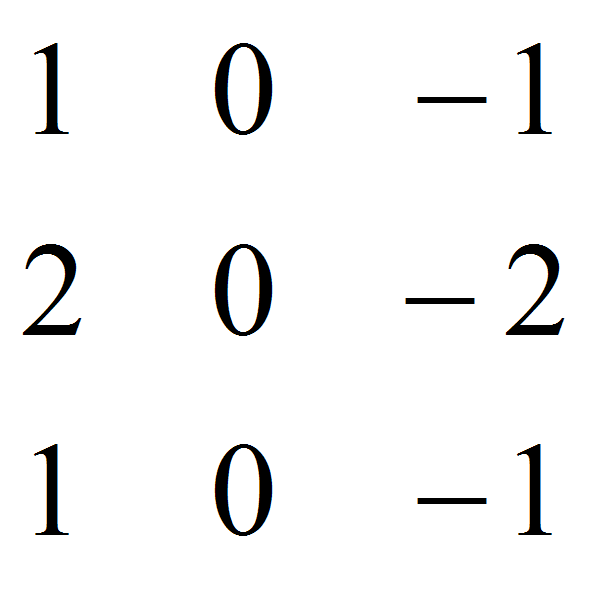
\includegraphics[width=1.87cm,height=1.87cm]{fig/CMCIBasicCourse201102-img108.png}
\[
 \begin{matrix}
  1 & 0 & -1 \\
  2 & 0 & -2 \\
  1 & 0 & -1
 \end{matrix}
\]
Be sure to make space between elements. Then to the duplicated image,
apply convolution with the following kernel:

%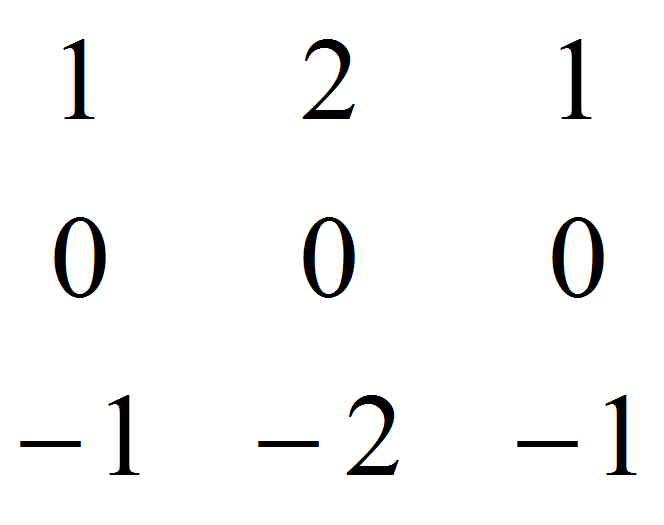
\includegraphics[width=2.364cm,height=1.87cm]{fig/CMCIBasicCourse201102-img109.png}
\[
 \begin{matrix}
  1 & 2 & 1 \\
  0 & 0 & 0 \\
  -1 & -2 & -1
 \end{matrix}
\]

Now we must get the root square of the sum of squared of each image,
which is

$Result =(microtubule.tif^{2}+ microtubule-1.tif^{2})^{0.5}$

For this calculation, one could use ImageMath function in ImageJ or ImageExpression Parser in Fiji. Depending on your setup, please do one of the following two ways. 

\begin{quote}
\textbf{ImageJ, by ImageMath}

Each image can be squared by \ijmenu{[Process > Math > Square]}. 
Then to squared images, do \ijmenu{[Process > Image Calculator]} for the addition of two squared images. This command pops up a window like below. 

%figure
\begin{figure}[htbp]
\begin{center}
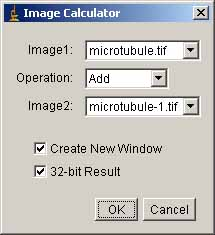
\includegraphics[width=4cm]{fig/CMCIBasicCourse201102-img110.jpg}
\caption{ Image Calculation}
\label{fig:ImageCalculatorDialog}
\end{center}
\end{figure}

From the pull down menu, select \textbf{microtubule.tif} and \textbf{microtubule-1.tif}. Don't forget to check \ijmenu{create new window} and \ijmenu{32-bit results}. Then click OK.
There will be a new window. To this new image titled \textbf{result of microtubule} do
\ijmenu{[Process > Math > Square Root]} for the final calculation. 
You probably would see only black frame, this is
because 32-bit image is not properly scaled and you need to adjust LUT.
To do so, do \ijmenu{[Image > Adjust > Brightness/Contrast] }
and in the Brightness \& Contrast window, click \ijmenu{Auto} to auto-scale the LUT.


\textbf{Fiji, by Image Expression Parser}

To do complex calculation between two images, Image Expression
parser could be used. Select \ijmenu{[Process > Image Expression Parser]}. Input
following in the Expression field:

\ilcom{\ \ sqrt(A\textasciicircum2+B\textasciicircum2)}


Then Choose \textbf{microtuble.tif} for "A"
and \textbf{microtubule-1.tif} (duplicate) for
"B". B might not be shown at the
start up. To show B selection field, click
"\ldots" button at bottom-left corner.
%figure
\begin{figure}[htbp]
\begin{center}
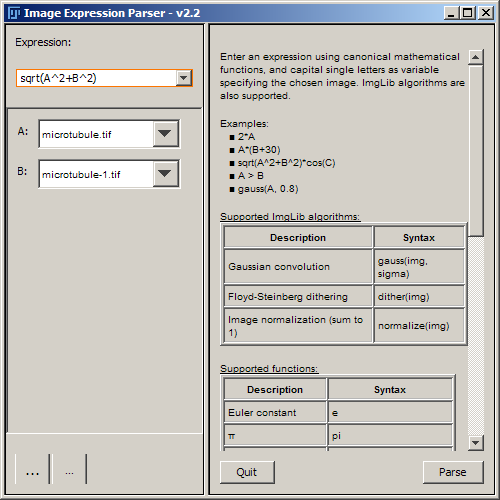
\includegraphics[width=10cm]{fig/CMCIBasicCourse201102-img111.png}
\caption{ Image Expression Parser (Fiji)}
\label{fig:ImageExpressionParser}
\end{center}
\end{figure}

\end{quote}

To compare the original and the edge detected images, go back to the
image \textbf{microtubule} and do
\ijmenu{[File > Revert]}. Then with "Result of Microtubule" do \ijmenu{[Image > Type > 8-bit]} 
to scale down the bit-depth. Merge the images by
\ijmenu{[Image > Color > RGB Merge\ldots]}.
In the following dialog window, choose appropriate color for each
image such as shown below. 

%double figure
\begin{figure}[H]
\centering
\subfloat[]{\label{fig:img112}
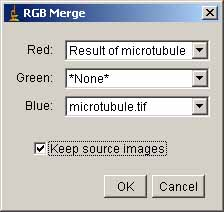
\includegraphics[height=3cm]{fig/CMCIBasicCourse201102-img112.jpg}
}
\subfloat[]{\label{fig:img113}
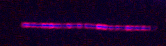
\includegraphics[width=8cm]{fig/CMCIBasicCourse201102-img113.png}
}
\caption{ RGB merge of detected edge over the original
image. (a) Dialog for assigning channels. (b) Example of merged color image, with original image in blue and edge-detected image in red}
\label{fig:EdgeDetectChannelMerging}
\end{figure} 

\end{indentexercise}

\subsection{Morphological Watershed }
\label{sec:Watershed}
In the previous sections, we discussed segmentation based on thresholding and edge detection. Morphological watersheds provide another way to segment objects. One advantage of the watershed algorithm is that it outputs continuous segmentation boundaries and often tends to produce stable segmentation results. In ImageJ, watershed algorithm could be found at \ijmenu{[Process > Binary > Watershed]}.

To understand the watershed transform we view a grayscale image as a
topological surface, where the values of f(x,y) correspond to heights:

%double figure
\begin{figure}[htbp]
\centering
\subfloat[]{\label{fig:img114}
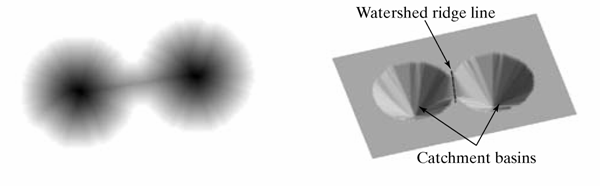
\includegraphics[width=8cm]{fig/CMCIBasicCourse201102-img114.png}
}
\subfloat[]{\label{fig:img115}
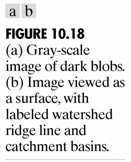
\includegraphics[width=2.3cm]{fig/CMCIBasicCourse201102-img115.png}
}
\caption{ Watershed Principle}
\label{fig:WatershedPrinciple}
\end{figure} 

Consider the topographic surface on the right. Water would collect in
one of the two catchment basins. Water falling on the watershed ridge
line separating the two basins would be equally likely to collect into
either of the two catchment basins. Watershed algorithms then find the
catchment basins and the ridge lines in an image 
(Fig. \ref{fig:WatershedPrinciple}, \ref{fig:img117}).

The algorithm works as follows: Suppose a hole is punched at each
regional local minimum and the entire topography is flooded from below
by letting the water rise through the holes at a uniform rate. Pixels
below the water level at a given time are marked as flooded. When we
raise the water level incrementally, the flooded regions will grow in
size. Eventually, the water will rise to a level where two flooded
regions from separate catchment basins merge. When this occurs,
the algorithm constructs a one-pixel thick dam that separates the two
regions. The flooding continues until the entire image is segmented
into separate catchment basins divided by watershed ridge lines.

\begin{indentexercise}{1}
Open binary image \textbf{Circles.tif} (Fig.~\ref{fig:img116}). You
see two circles fused. Such situation often occurs with cells or
organelle, and you might want to simply separate them as different
objects. 

%figure
\begin{figure}[htbp]
\begin{center}

\includegraphics[width=2.381cm,height=2.408cm]{fig/CMCIBasicCourse201102-img116.png}
\caption{ Circles.tif}
\label{fig:img116}
\end{center}
\end{figure}

Do \ijmenu{[Process > Binary > Watershed]}. You will see that the two circles are separated at the
constricted part of the fused circles. 
\end{indentexercise}

If you want to know a bit more details, read the following quote how ImageJ does this.
\begin{quote}
Watershed segmentation is a way of automatically separating or cutting
apart particles that touch. It first calculates the Euclidean distance
map (EDM) and finds the ultimate eroded points (UEPs). It then dilates
each of the UEPs (the peaks or local maxima of the EDM) as far as
possible - either until the edge of the particle is reached, or the
edge of the region of another (growing) UEP. Watershed segmentation
works best for smooth convex objects that don't
overlap too much. (quote from ImageJ web site) 
\end{quote}
%figure
\begin{figure}[htbp]
\begin{center}
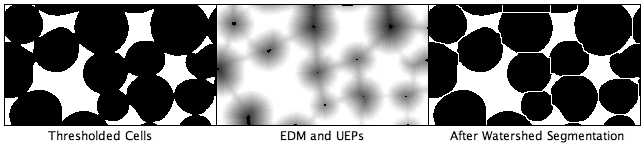
\includegraphics[width=13.418cm,height=2.701cm]{fig/CMCIBasicCourse201102-img117.png}
\caption{ Watershed Segmentation}
\label{fig:img117}
\end{center}
\end{figure}

ImageJ first computes the distance transform on the binary image. The distance transform of
a binary image is the distance from every pixel to the nearest nonzero-valued, or background, pixel, as example in Fig. \ref{fig:img118} shows.
%figure
\begin{figure}[htbp]
\begin{center}
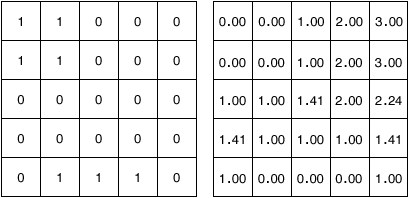
\includegraphics[width=10.85cm,height=5.242cm]{fig/CMCIBasicCourse201102-img118.png}
\caption{ A small binary image (left) and its distance transform (right)}
\label{fig:img118}
\end{center}
\end{figure}


\subsection{Particle Analysis}

After the segmentation, the objects could be analyzed for extracting various
parameters about objects. A powerful function in ImageJ for this purpose is the particle
analysis function. It counts the number of objects (particles) in the
image, extracts morphological parameters, measures intensity\ldots and
so on. For details on extractable parameters, refer to Appendix
\ref{app2}. Here, we take an example to learn the basic use of
this function.  

\begin{indentexercise}{1}
Single Particle Detection

Load \textbf{Circles.tif} and segment two circles by watershed operation
as we did in the previous section. Then select the Wand Tool 

\includegraphics[width=0.5cm]{fig/CMCIBasicCourse201102-img119.png}
 from the tool bar. Click one of the circles. Check that a ROI is
automatically highlighted at the edge of the circle.
\end{indentexercise}

Automatic detection is done by pixel similarity principle. In the above
case using the wand tool, computer searches for pixels in the
surrounding of the clicked pixel for similarity in the pixel value.
Similar pixels will be labeled. Then in the next round, computer
searches for each of the labeled pixel for similar surrounding. This
continues until searching hits the boundary. Particle analysis uses the
same strategy, but there will be specific labeling for each particle.

\begin{indentexercise}{2}
\item Multiple Particle Analysis: Open \textbf{rice.tif}. Before applying particle analysis, target
particles must be segmented by image threshold. Try thresholding the
image\ldots What you would find out immediately is that there is shading in
the image that rice can not be uniformly selected by thresholded. For this reason, do the
background subtraction as we already did in \ref{exer:removerice}. 
We then work with the subtracted image in the
following.

Set Threshold again, and then click ``Apply'' in the Threshold dialog window. 
The image then should be black and white. This binarized (segmented) image 
will be used as a reference for setting boundary of each rice grain. 

Open file \textbf{rice.tif} again. Since there is already a window with the same title, this second one 
should have a title ``rice-1.tif''. By having this original image, boundaries that will be set using the binarized image 
will be "redirected" when measurement is actually taking place\footnote{ It is also possible to 
do the measurement without redirecting: for example, you could simply image-threshold, and while the image is highlighted with red, (do not click Apply button) and do ``Analyze particle''. This will then detect particles which are highlighted.}. 

Before doing particle analysis, you must specify what you want to
measure for each particle through \ijmenu{[Analysis > Set
Measurements]}. Select Area, Circularity, Centroid and Perimeter
(details on these parameters are written in Appendix \ref{app2}).
In addition, set ``redirect to'' to the original image (rice-1.tif) so
that the measurement will be done with the original image and not with 
the thresholded image. 

Activate the thresholded image, and then do \ijmenu{[Analyze > Analyze
Particles\ldots]}. A dialog window pops up. Input following
parameters:
\begin{itemize}
\item Size: "0-200", i.e. size above 200 pixel area will be excluded from the measurement
\item Circularity: use default "0-1.0"
\item Show: Outline
\item Check box:
\begin{itemize} 
\item Check "Display Results" to display the result table.
\item Check "Clear Results" to refresh the measurement recordings.
\item Check "Exclude on Edges" to exclude particles touching the edge of the image. 
\end{itemize}
\end{itemize}
Then Click "OK". Two windows pop up. One
is the outline image of the measured particles, with number labels.
These numbers correspond to the numbers you see at the left most column
in the result window, which also popped up. Examine the outline image.
At the bottom, there seems to be some particles which are counted but
only part of the particles are included. 

%figure
\begin{figure}[H]
\begin{center}
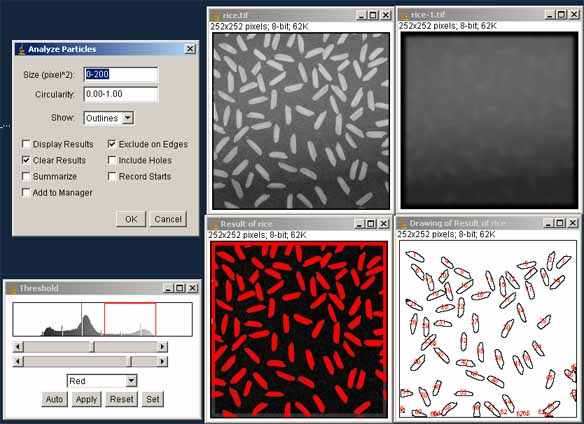
\includegraphics[width=10cm]{fig/CMCIBasicCourse201102-img120.jpg}
\caption{ Multiple particle Analysis}
\label{fig:img120}
\end{center}
\end{figure}

\textbf{QUESTION}: How can we eliminate edge-touching particles from the
analysis? Which parameter in the "Analyze
Particle" dialog should we change? Try again with
different parameter values.
\end{indentexercise}

\subsection{Machine Learning: Trainable Segmentation}

Segmentation could also be done by letting computer to learn what you
think as signal and background. To do so, one could use machine
learning algorithms. 

We use the \textbf{Trainable Segmentation plugin}.
In brief, you manually mark what you decide as signal and background, and then
let the plugin to "Train"
a classifier. The plugin studies your markings by combining many possible features and it comes up with a model to
categorize each pixel into classes to output a segmented image. 
 
When you start the plugin, you
will see a window with the image you want to segment, and buttons in the
surrounding. The panel in left side is for commands, and the panel in right
side is for assigning your markings of either signal or background. There
are only two classes on start up but you could add more classes (e.g.
signal 1, signal 2, background) by clicking ``create new
class" in the left panel (Fig. \ref{fig:img121}). 
%figure
\begin{figure}[H]
\begin{center}
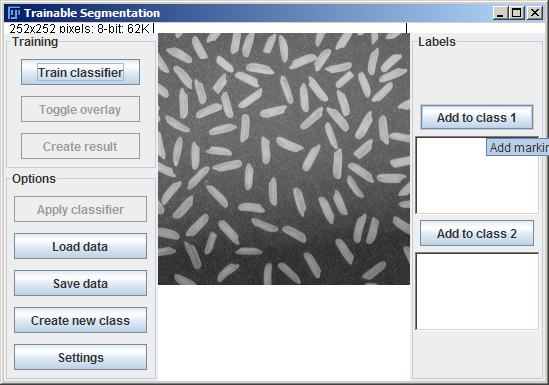
\includegraphics[width=9.947cm,height=6.872cm]{fig/CMCIBasicCourse201102-img121.png}
\caption{ Trainable Segmentation Window}
\label{fig:img121}
\end{center}
\end{figure}

\begin{indentexercise}{1}
(This exercise is only available with the Fiji distribution)

Open \textbf{rice.tif} and then select 

\ijmenu{[Plugins > Segmentation > Trainable Segmentation]}. 

Your task here is to segment rice grains using trainable segmentation. Zoom up the image
using magnifying tool as usual image. Then choose free hand ROI tool,
start marking a rice grain. 

If you are satisfied with ROI, then click
\ijmenu{Add to Class1}. Then
again using freehand ROI tool, mark background. Then add this another
class by \ijmenu{Add to Class2}. Your trainable segmentation window should look
something like Fig. \ref{fig:img122}. 

%figure
\begin{figure}[htbp]
\begin{center}
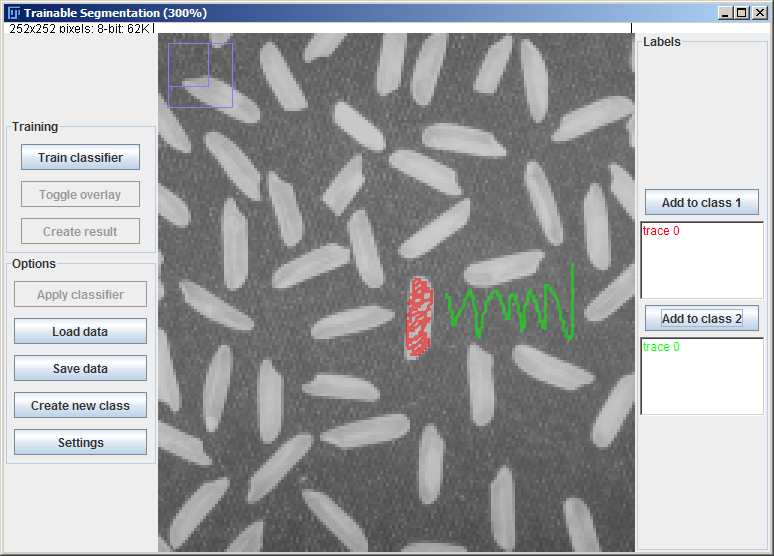
\includegraphics[width=9.001cm,height=6.447cm]{fig/CMCIBasicCourse201102-img122.png}
\caption{ Marking signal and background}
\label{fig:img122}
\end{center}
\end{figure}

Click \ijmenu{Train Classifier} in the left panel, then the calculation starts, which takes for a while. When
calculation finishes, you will see that most of rice grains are overlaid in red and background in green (Fig. \ref{fig:img123}). Zoom out the image and check again. You might see that some rice grains are not segmented well -- so we should train more. Use freehand ROI tool to mark that was unfortunately either categorized
as background or partly missed, and add it to class 1 (\ijmenu{Add to Class 1}). Then \ijmenu{Train
classifier}, check the segmentation results\ldots You
could repeat such marking and training until you get a satisfactory
segmentation result (Fig.~\ref{fig:img123}). 

TIP: You could delete specific trace already
listed in Class listing by double clicking it.

%figure
\begin{figure}[htbp]
\begin{center}
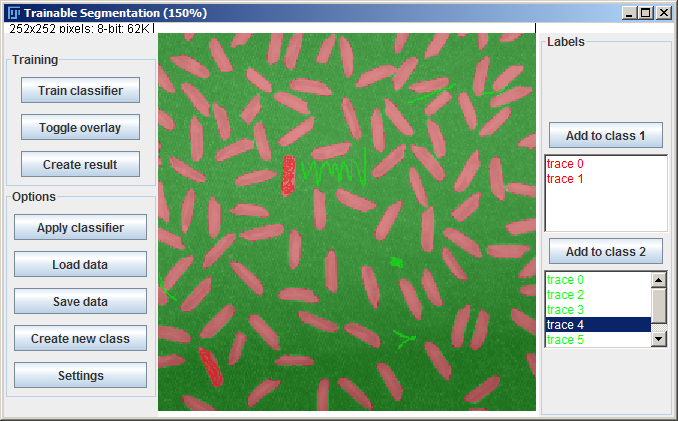
\includegraphics[width=9cm]{fig/CMCIBasicCourse201102-img123.png}
\caption{ After first round of trainable segmentation.}
\label{fig:img123}
\end{center}
\end{figure}

To create segmented image, click \ijmenu{Create result}. 
A separate window with segmented image will open (Fig. \ref{fig:img124}). 

%figure
\begin{figure}[htbp]
\begin{center}
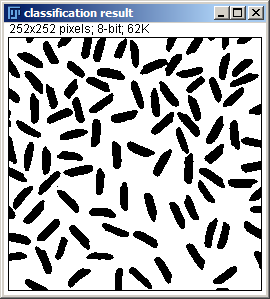
\includegraphics[width=6cm]{fig/CMCIBasicCourse201102-img124.png}
\caption{ Segmentation Result of Trainable Segmentation PlugIn}
\label{fig:img124}
\end{center}
\end{figure}

During the training, a set of feature data and its classes are generated. To save the data used for training, click \ijmenu{save data}. Saved *.arff file could be loaded later to segment another image 
(should be rice in this case, of course!) using \ijmenu{Load data} button.

\textbf{OPTIONAL} : Segmented image could be used as a mask to analyze original image. 
To do so, open both the original \textbf{rice.tif} image and binary image (segmented rice.tif image).
Then \ijmenu{[Analyze > Set Measurement]}, and set \ijmenu{redirect to} drop down menu to
original image (rice.tif). Then activate the segmented image window, threshold the image (but do not
"apply"), and do particle analysis. 
Detection of particles are done in the segmented image, and
measurements will be redirected to corresponding particle areas in the
original image.  
\end{indentexercise}

\clearpage


\subsection{ASSIGNMENTS}

\textbf{\sffamily
Assignment 1-4-1 Quantum dots.}

Devise a segmentation strategy to segment
the following image of quantum dots (quantumdots.tif). Extract the
following parameters from the image: 
\begin{enumerate} 
\item number of dots
\item histogram of areas
\item histogram of integrated densities 
\end{enumerate}
You can draw histogram of the results in the "Results" window by using a
function associated with the Result window \ijmenu{[Edit > Distribution\ldots]}.\\

{\centering 
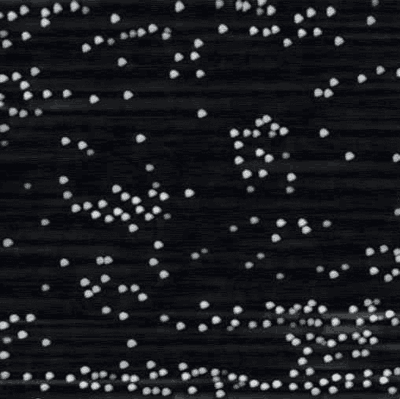
\includegraphics[width=7cm]{fig/CMCIBasicCourse201102-img125.png}
\par}

\textbf{\sffamily
Assignment 1-4-2  DIC images of cells. }

Find the boundary of this cell (dic\_cell.tif) using any of your favorite image segmentation techniques.\\

{\centering 
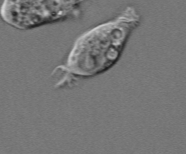
\includegraphics[width=7cm]{fig/CMCIBasicCourse201102-img126.png}
\par}

\textbf{\sffamily
Assignment 1-4-3  Actin filaments.}

Devise an image processing strategy to
obtain the distribution of filaments from this image (actin.tif), and subsequently
calculate 
\begin{enumerate}
\item the mean filament length
\item the variance in filament length
\item the number of filaments. 
\end{enumerate}
Note: image segmentation may be complicated by the low light levels in the image. \\

{\centering 
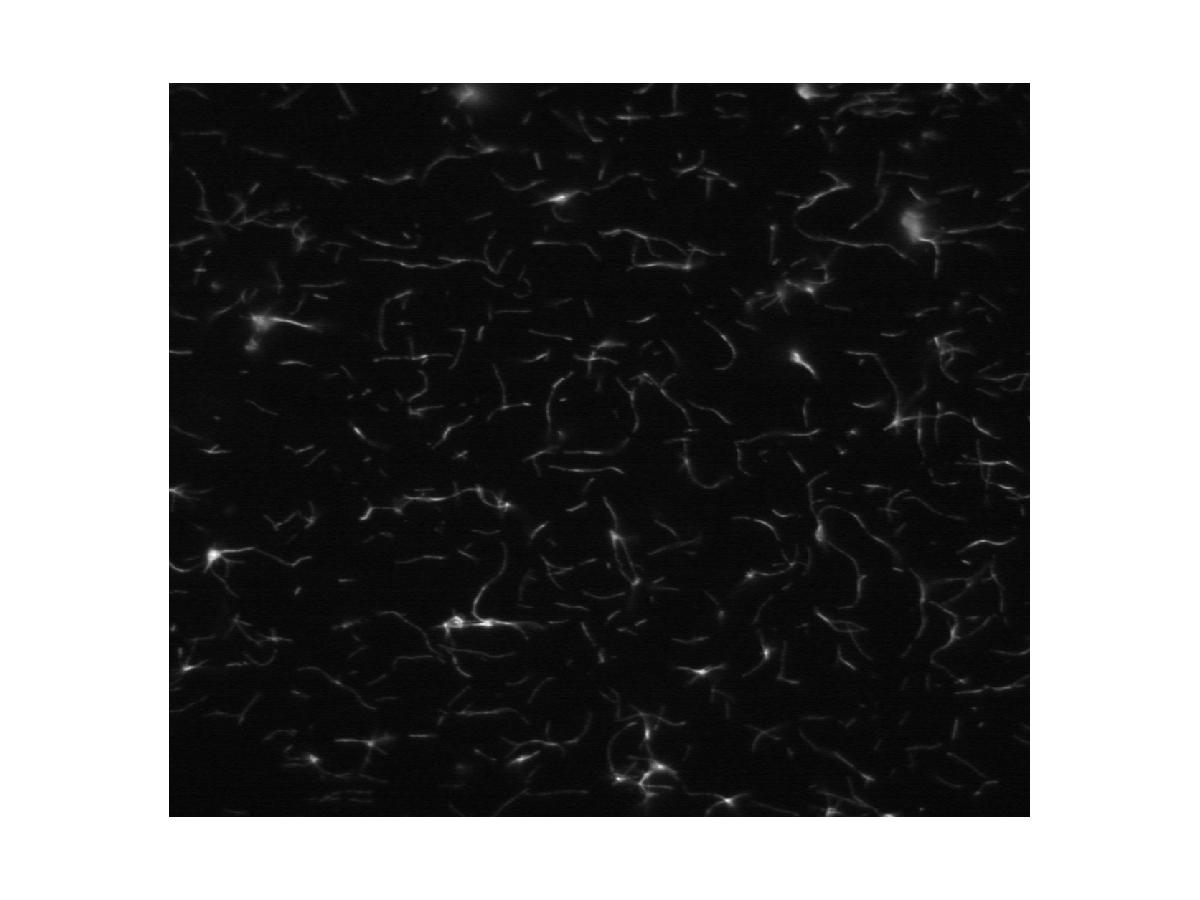
\includegraphics[width=10cm]{fig/CMCIBasicCourse201102-img127.jpg}
\par}

\textbf{\sffamily
Assignment 1-4-4  Fixed cells.}

Here are some cells that are fixed and
stained for actin (red), tubulin (green) DNA (blue), and a histone
marker (not shown, 4color\_cells). Devise an image processing strategy to segment
the cells. You may operate on any of the color channels in the image
(or a multiple of them). This problem is especially tricky because
many of the cells are touching.  \\

{\centering 
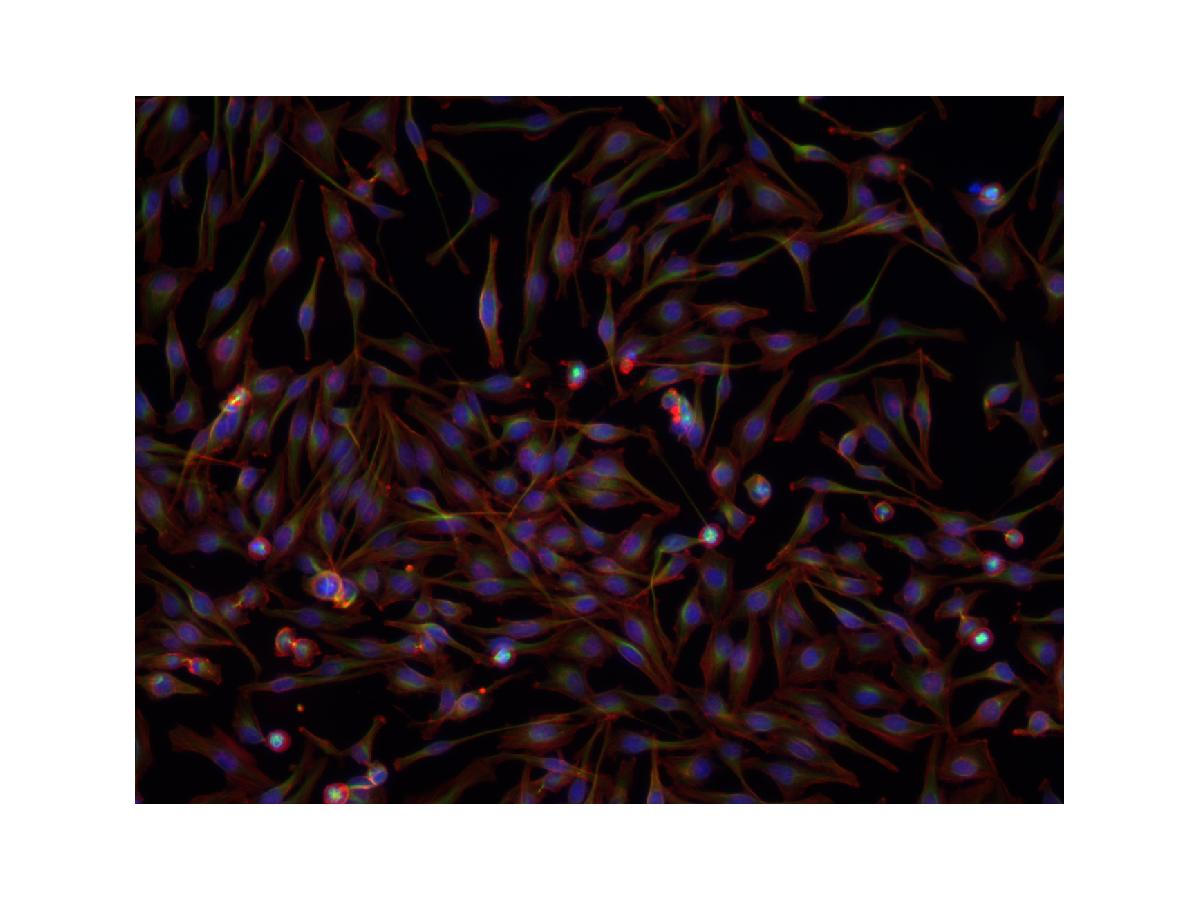
\includegraphics[width=10cm]{fig/CMCIBasicCourse201102-img128.jpg}
\par}

